% Provenance (never printed): see sources/outline_sources.md (Year 2: index minerals and zones,
% geothermometers and geobarometers, prograde and retrograde paths, metamorphic series,
% ultrahigh-pressure rocks and exhumation, ocean-floor metamorphism). Garnet-biotite
% calibration refitted from the Ferry and Spear (1978) brackets tabulated by Holdaway et al.
% (1997); GASP from Koziol and Newton (1988); thickening model after England and Thompson
% (1984) in figdata/bachelor-2/ptpaths.py; exercise and problem values in the Book 4 scratch
% calculators calc/ch11.py and calc/ch11b.py.
\chapter{Termobarometri dan Lintasan P--T--t}\label{ch:b2:pt-paths}

Sebutir garnet selebar beberapa milimeter, yang tumbuh di dalam sekis, menyimpan di intinya komposisi
yang dimilikinya ketika mulai tumbuh dan di tepinya komposisi yang dimilikinya ketika berhenti tumbuh. Setiap
zona setimbang dengan biotit dan plagioklas di sekelilingnya pada saat itu, dan
cara besi, magnesium, dan kalsium terbagi di antara mineral-mineral ini bergantung pada suhu
dan tekanan. Bila dibaca dengan termodinamika bab sebelumnya, garnet menunjukkan seberapa
dalam batuannya terkubur dan seberapa panas batuan itu; bila diberi umur, garnet menunjukkan kapan, dan seberapa cepat
batuan itu naik kembali. Bab ini mengubah mineral metamorf menjadi termometer, barometer,
dan jam, lalu mengikuti sebuah batuan di sepanjang lintasannya menembus kerak.

\begin{recall}
\textbf{Dari volume sekolah menengah atas}: derajat \omterm{def:b2:metamorphic-facies:metamorphism}{metamorfisme}, mineral indeks, dan isograd.
\textbf{Dari volume Tahun 1}: geoterm dan produksi panas radiogenik; kerak
benua yang tebalnya sekitar \qty{35}{km}; penentuan umur radiometrik, suhu penutupan
suatu mineral dan umur pendinginan yang diberikannya; kerak samudra dan \omterm{def:b2:mantle-melting:peridotites}{peridotitnya}.
\textbf{Dari buku-buku fisika}: persamaan kalor $\partial T/\partial t = \kappa\,
\partial^2 T/\partial z^2$ dan difusivitas termal $\kappa$. \textbf{Dari buku-buku
kimia}: tetapan kesetimbangan, $\Delta_r G^\circ + RT\ln K = 0$, dan aktivitas dalam
larutan ideal. \textbf{Dari \cref{ch:b2:metamorphic-facies}}: \omterm{def:b2:metamorphic-facies:reaction}{reaksi metamorfik},
\omterm{def:b2:metamorphic-facies:clapeyron}{kemiringan Clapeyron}, diagram \ce{Al2SiO5}, dan fasies.
\end{recall}
% ledger: prem:moho-average

\section{Zona metamorfik}\label{sec:b2:pt-paths:zones}

Di batu lumpur Dataran Tinggi Skotlandia, George Barrow memetakan pada tahun 1890-an serangkaian
zona, masing-masing ditandai oleh kemunculan pertama mineral indeks yang baru. Ke arah derajat
yang lebih tinggi, klorit berturut-turut disertai biotit, garnet, staurolit, kianit, dan silimanit;
di penampang-penampang tipenya, zona garnet sampai silimanit terbentuk pada sekitar 500 sampai
\qty{650}{\celsius} dan 5 sampai \qty{7}{kbar}.
% ledger: iugs:barrow, barrow1893:paper, earle:regional

\begin{definition}[Zona Barrow; gradien metamorfik lapangan]\label{def:b2:pt-paths:barrovian}
Yang disebut \emph{zona Barrow}\index{zona Barrow} adalah zona-zona metamorfik
\omterm{def:b2:metamorphic-facies:protoliths}{metapelit} dengan urutan klorit, biotit, garnet, staurolit, kianit, silimanit,
masing-masing dimulai pada isograd mineral indeksnya. Yang disebut \emph{gradien metamorfik
lapangan}\index{gradien metamorfik lapangan} suatu wilayah adalah kurva, pada bidang
tekanan--suhu, yang melalui kondisi puncak yang direkam batuan-batuannya di
tempat batuan itu kini tersingkap.
\end{definition}

Setiap titik pada gradien lapangan berasal dari batuan yang berbeda, dan setiap batuan mencapai
puncaknya sendiri pada waktunya sendiri: gradien lapangan bukanlah geoterm pada satu saat mana pun, juga bukan
lintasan satu batuan mana pun. Gradien itu adalah jejak yang ditinggalkan puncak-puncak itu pada permukaan erosi masa kini.

\begin{omfigure}
\centering
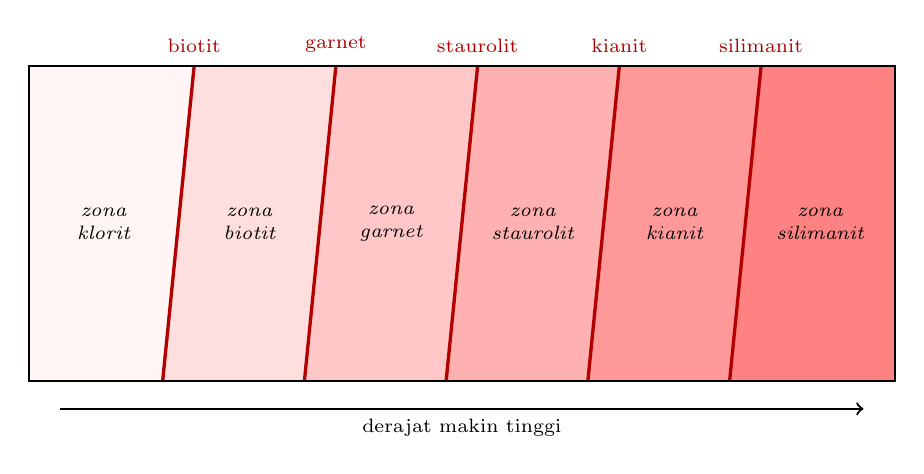
\begin{tikzpicture}[x=1cm, y=1cm]
\def\iso{{0,1.9,3.7,5.5,7.3,9.1,11}}
\foreach \i [evaluate=\i as \op using 4+9*\i] in {0,...,5} {
  \pgfmathsetmacro{\xa}{\iso[\i]}\pgfmathsetmacro{\xb}{\iso[\i+1]}
  \pgfmathsetmacro{\da}{(\i>0)*0.2}\pgfmathsetmacro{\db}{(\i<5)*0.2}
  \fill[red!\op!white] (\xa-\da,0) -- (\xb-\db,0) -- (\xb+\db,4) -- (\xa+\da,4) -- cycle;
}
\foreach \x/\n in {1.9/biotit, 3.7/garnet, 5.5/staurolit, 7.3/kianit, 9.1/silimanit} {
  \draw[very thick, red!70!black] (\x-0.2,0) -- (\x+0.2,4);
  \node[font=\scriptsize, red!70!black, anchor=south] at (\x+0.2,4.05) {\n};
}
\draw[thick] (0,0) rectangle (11,4);
\foreach \x/\z in {0.95/klorit, 2.8/biotit, 4.6/garnet, 6.4/staurolit, 8.2/kianit, 10.05/silimanit}
  \node[font=\scriptsize\itshape, align=center] at (\x,2) {zona\\\z};
\draw[->, thick] (0.4,-0.35) -- node[below, font=\scriptsize] {derajat makin tinggi} (10.6,-0.35);
\end{tikzpicture}
\par\smallskip{\small \omterm{def:b2:pt-paths:barrovian}{Zona Barrow} pada peta, skematis. Setiap isograd (garis merah, yang namanya tertera
di atas peta) adalah garis tempat mineral indeksnya pertama kali muncul; derajat \omterm{def:b2:metamorphic-facies:metamorphism}{metamorfisme}, dan pekatnya
arsiran, naik ke kanan. Setiap zona dinamai menurut mineral yang muncul pada
batas derajat rendahnya.}
\end{omfigure}
% ledger: iugs:barrow

Isograd dipetakan dari kemunculan mineral, dan baru menjadi kondisi tekanan dan
suhu setelah reaksi di baliknya diketahui. Untuk melangkah lebih jauh, kita perlu mengukur
suhu dan tekanan dalam satu batuan.

\section{Termometer dan barometer}\label{sec:b2:pt-paths:thermobarometry}

\begin{definition}[Geotermometer; geobarometer; reaksi pertukaran; reaksi transfer neto]\label{def:b2:pt-paths:thermobarometry}
Yang disebut \emph{geotermometer}\index{geotermometer} (\emph{geobarometer}\index{geobarometer}) adalah
kesetimbangan di antara mineral-mineral yang posisinya terutama bergantung pada suhu (tekanan), sehingga
komposisi mineral-mineral itu memberikan suhu (tekanan) kesetimbangan terakhirnya. Yang disebut
\emph{reaksi pertukaran}\index{reaksi pertukaran} adalah reaksi yang menukar dua unsur
di antara dua mineral, seperti besi dan magnesium di antara garnet dan biotit, tanpa
menciptakan atau memusnahkan salah satu mineral itu. Yang disebut \emph{reaksi transfer neto}\index{reaksi transfer neto}
adalah reaksi yang membentuk sebagian mineral dengan mengorbankan mineral lain.
\end{definition}

Termometer \omterm{def:b2:metamorphic-facies:protoliths}{metapelit} yang paling luas dipakai adalah pertukaran besi dan magnesium
antara garnet dan biotit,
\[
\ce{Fe3Al2Si3O12 + KMg3AlSi3O10(OH)2 <=> Mg3Al2Si3O12 + KFe3AlSi3O10(OH)2},
\]
yaitu almandin ditambah flogopit menghasilkan pirop ditambah anit. Misalkan $X_{\text{Mg}}$ dan $X_{\text{Fe}}$
fraksi situs yang diisi magnesium dan besi dalam setiap mineral, dan
\[
K_D = \frac{(X_{\text{Mg}}/X_{\text{Fe}})_{\text{garnet}}}{(X_{\text{Mg}}/X_{\text{Fe}})_{\text{biotit}}}.
\]
% ledger: h97:fs-reaction

\begin{proposition}[Sebuah kesetimbangan pertukaran]\label{prop:b2:pt-paths:exchange}
Jika garnet dan biotit adalah larutan ideal dan $\Delta_r H$, $\Delta_r S$, dan $\Delta_r V$
reaksi di atas konstan, maka pada kesetimbangan
\[
3RT\ln K_D = -(\Delta_r H + P\,\Delta_r V) + T\,\Delta_r S,
\qquad\text{jadi}\qquad
T = \frac{\Delta_r H + P\,\Delta_r V}{\Delta_r S - 3R\ln K_D}.
\]
\end{proposition}

\begin{proof}
Setiap mineral memiliki tiga situs untuk besi atau magnesium. Dalam larutan ideal, aktivitas
suatu anggota ujung adalah hasil kali fraksi situs yang diisinya: $a_{\text{pirop}} =
X_{\text{Mg}}^3$ dalam garnet, dan seterusnya. Karena itu tetapan kesetimbangannya adalah
\[
K = \frac{a_{\text{pirop}}\,a_{\text{anit}}}{a_{\text{almandin}}\,a_{\text{flogopit}}}
= \frac{X_{\text{Mg,grt}}^3\,X_{\text{Fe,bt}}^3}{X_{\text{Fe,grt}}^3\,X_{\text{Mg,bt}}^3} = K_D^3 .
\]
Pada kesetimbangan $\Delta_r G^\circ(T, P) + RT\ln K = 0$, dengan $\Delta_r G^\circ = \Delta_r H -
T\,\Delta_r S + P\,\Delta_r V$ (angka 1 dalam $P - 1$ diabaikan), yang memberikan persamaan pertama;
penyelesaiannya untuk $T$ memberikan persamaan kedua.
\end{proof}

Konstanta-konstantanya berasal dari percobaan tempat garnet dan biotit sintetis bertukar besi
dan magnesium pada suhu yang diketahui dan \qty{2.07}{kbar}. Dua belas rentang semacam itu, dari 550 sampai
\qty{800}{\celsius}, yang diplot sebagai $\ln K_D$ terhadap $1/T$, jatuh di dekat sebuah garis (gambar
di bawah); bila dicocokkan dengan kuadrat terkecil dengan $\Delta_r V = \qty{0.311}{J.bar^{-1}}$, rentang-rentang itu memberikan
$\Delta_r H = \qty{52630}{J}$ dan $\Delta_r S = \qty{20.19}{J.K^{-1}}$, nilai-nilai dari
perhitungan ulang terbitan atas data yang sama. Pada suhu yang lebih tinggi, rasio $K_D$ naik
mendekati 1: garnet mengambil bagian magnesium yang lebih besar.
% ledger: h97:fs-data, h97:ideal, h97:fs-reaction

\begin{omfigure}
\centering
\begin{tikzpicture}
\begin{axis}[omrecord, width=0.62\linewidth, height=5.2cm,
  xmin=0.9, xmax=1.25, ymin=-1.9, ymax=-1.1,
  xlabel={$1000/T$ (\unit{K^{-1}})}, ylabel={$\ln K_D$},
  tick label style={font=\scriptsize}, label style={font=\small},
  x tick label style={/pgf/number format/.cd, fixed, precision=2}]
\addplot[only marks, mark=*, mark size=1.6pt, blue!70!black]
  table[x expr={1000/(\thisrow{T_C}+273.15)}, y=lnKD] {figdata/out/bachelor-2-ptpaths-fs.dat};
\addplot[thick, red!75!black, domain=0.9:1.25, samples=2] {(-52630-2070*0.311)/(3*8.31441)*x/1000 + 20.19/(3*8.31441)};
\end{axis}
\end{tikzpicture}
\par\smallskip{\small Pertukaran garnet--biotit: dua belas rentang eksperimental pada
\qty{2.07}{kbar} (biru, sebagaimana ditabulasikan oleh Holdaway dan kawan-kawan, 1997) dan garis
proposisi dengan $\Delta_r H$ dan $\Delta_r S$ hasil pencocokan (merah).}
\end{omfigure}
% ledger: h97:fs-data, h97:ideal

Untuk $K_D = 0.18$ pada \qty{5}{kbar}, $T = (52630 + 0.311\times5000)/(20.19 - 3\times8.314
\times\ln 0.18) = 54185/62.96 = \qty{861}{K}$, atau \qty{587}{\celsius}. Satu kilobar lagi
menambahkan $0.311\times1000/62.96 = \qty{4.9}{K}$: reaksi itu menukar ion bermuatan sama
di antara situs yang ukurannya hampir sama, perubahan volumenya kecil, dan tekanan hampir tidak
berpengaruh. Itulah yang membuatnya menjadi termometer.

Barometer memerlukan kebalikannya: reaksi dengan perubahan volume yang besar. \omterm{def:b2:pt-paths:thermobarometry}{Reaksi
transfer neto}
\[
\ce{3 CaAl2Si2O8 <=> Ca3Al2Si3O12 + 2 Al2SiO5 + SiO2},
\]
yaitu anortit menghasilkan grosular, kianit, dan kuarsa, memampatkan atom-atom tiga feldspar ke dalam
mineral yang lebih rapat: $\Delta_r V = \qty{-6.21}{J.bar^{-1}}$, dua puluh kali perubahan volume \omterm{def:b2:pt-paths:thermobarometry}{reaksi pertukaran} tadi.
Kesetimbangan anggota-ujungnya, yang dibalikkan dalam percobaan pada 900 sampai \qty{1250}{\celsius} dan 19
sampai \qty{28}{kbar}, berjalan di sepanjang
\[
P_0 = 22.80\,T - 1093 \qquad (P_0 \text{ dalam bar}, T \text{ dalam } \unit{\celsius}).
\]
Dalam batuan, grosular hanyalah bagian kecil garnet dan anortit adalah bagian dari
plagioklas. Dengan aktivitas ideal, $a_{\text{grosular}} = X_{\text{Ca,grt}}^3$ dan
$a_{\text{anortit}} = X_{\text{an}}$, syarat $\Delta_r G^\circ + RT\ln K = 0$
yang dituliskan pada $P$ dan pada $P_0$ memberikan
\[
P = P_0 + \frac{RT}{6.21}\,\ln\frac{X_{\text{Ca,grt}}^3}{X_{\text{an}}^3}
\qquad (T \text{ dalam kelvin pada suku kedua}).
\]
\omterm{def:b2:pt-paths:thermobarometry}{Geobarometer} ini, yang dinamai GASP menurut empat mineralnya (garnet, aluminosilikat, silika,
plagioklas), dapat dipakai di mana pun \omterm{def:b2:metamorphic-facies:protoliths}{metapelit} mengandung keempatnya.
% ledger: kn88:gasp, rh95:gb-gasp

\begin{method}[Suhu dan tekanan satu batuan]\label{met:b2:pt-paths:intersection}
(1) Ukurlah, pada mineral-mineral yang tumbuh bersama, komposisi yang diperlukan termometer dan
barometer. (2) Tebaklah suatu tekanan dan hitunglah suhunya dengan termometer.
(3) Pada suhu itu, hitunglah tekanannya dengan barometer. (4) Ulangi (2) dan (3)
sampai keduanya tidak berubah; dua atau tiga putaran sudah cukup, karena setiap persamaan hanya sedikit bergantung pada
variabel yang ditetapkan persamaan lainnya. Secara grafis, jawabannya adalah titik potong garis
termometer dengan garis barometer. (5) Rambatkan ketidakpastiannya: untuk
galat yang saling independen, $\sigma_T^2 = (\partial T/\partial\ln K_D)^2\sigma_{\ln K_D}^2 +
(\partial T/\partial P)^2\sigma_P^2$, dan dengan cara serupa untuk $P$.
\end{method}

\begin{omfigure}
\centering
\begin{tikzpicture}
\begin{axis}[omrecord, width=0.78\linewidth, height=6.4cm,
  xmin=400, xmax=800, ymin=0, ymax=12, xlabel={$T$ (\unit{\celsius})}, ylabel={$P$ (\unit{kbar})},
  tick label style={font=\scriptsize}, label style={font=\small}, clip=false]
\addplot[thick, red!75!black] table[x=kd12, y=P_kbar] {figdata/out/bachelor-2-ptpaths-gb.dat};
\addplot[thick, red!75!black] table[x=kd15, y=P_kbar] {figdata/out/bachelor-2-ptpaths-gb.dat};
\addplot[thick, red!75!black] table[x=kd18, y=P_kbar] {figdata/out/bachelor-2-ptpaths-gb.dat};
\addplot[thick, red!75!black] table[x=kd21, y=P_kbar] {figdata/out/bachelor-2-ptpaths-gb.dat};
\addplot[thick, red!75!black] table[x=kd24, y=P_kbar] {figdata/out/bachelor-2-ptpaths-gb.dat};
\addplot[thick, blue!70!black] table[x=T_C, y=r15] {figdata/out/bachelor-2-ptpaths-gasp.dat};
\addplot[thick, blue!70!black] table[x=T_C, y=r20] {figdata/out/bachelor-2-ptpaths-gasp.dat};
\addplot[thick, blue!70!black] table[x=T_C, y=r25] {figdata/out/bachelor-2-ptpaths-gasp.dat};
\addplot[thick, blue!70!black] table[x=T_C, y=r30] {figdata/out/bachelor-2-ptpaths-gasp.dat};
\node[font=\tiny, red!75!black, anchor=west] at (axis cs:452,0.5) {0.12};
\node[font=\tiny, red!75!black, anchor=west] at (axis cs:511,0.5) {0.15};
\node[font=\tiny, red!75!black, anchor=west] at (axis cs:568,0.5) {0.18};
\node[font=\tiny, red!75!black, anchor=west] at (axis cs:622,0.5) {0.21};
\node[font=\tiny, red!75!black, anchor=west] at (axis cs:675,0.5) {0.24};
\node[font=\tiny, blue!70!black, anchor=west] at (axis cs:802,8.97) {0.15};
\node[font=\tiny, blue!70!black, anchor=west] at (axis cs:802,10.21) {0.20};
\node[font=\tiny, blue!70!black, anchor=west] at (axis cs:802,11.17) {0.25};
\node[font=\tiny, blue!70!black, anchor=west] at (axis cs:802,11.96) {0.30};
\end{axis}
\end{tikzpicture}
\par\smallskip{\small Isoterm garnet--biotit (merah, curam, diberi label $K_D$) dan isobar
GASP (biru, diberi label di kanan dengan rasio $X_{\text{Ca}}/X_{\text{an}}$, yaitu
grosular dalam garnet terhadap anortit dalam plagioklas), dari kalibrasi subbab ini. Batuan yang mengandung kedua pasangan itu terletak
di titik potong kedua garisnya.}
\end{omfigure}
% ledger: h97:ideal, h97:fs-reaction, kn88:gasp

Garis-garis termometer hampir vertikal, garis-garis barometer miring: keduanya berpotongan dengan
sudut lebar, yang menjaga titik potong tetap teliti. Pencampuran ideal adalah penyederhanaan utama
bab ini. Garnet yang sebenarnya mengandung kalsium dan mangan, biotit yang sebenarnya mengandung aluminium,
titanium, dan besi feri, dan kalibrasi yang mengoreksinya menggeser suhu sebesar
puluhan derajat (di satu wilayah yang diteliti dengan baik, \qty{574}{\celsius}, bukan
\qty{530}{\celsius}); kalibrasi terbaik mengklaim ketidakpastian sekitar \qty{25}{\celsius}.
% ledger: h97:ideal, h97:corrections

\section{Lintasan tekanan--suhu}\label{sec:b2:pt-paths:paths}

Batuan tidak mencapai tekanan tertinggi dan suhu tertingginya pada saat yang sama.
Batuan itu terkubur dan terpanaskan, lalu terangkat kembali dan mendingin, dan mineral-mineralnya bereaksi di sepanjang
perjalanan itu.

\begin{definition}[Lintasan P--T; lintasan progradasi dan retrogradasi; kondisi puncak metamorfisme]\label{def:b2:pt-paths:paths}
Yang disebut \emph{lintasan P--T}\index{lintasan P--T} suatu batuan adalah urutan tekanan dan
suhu yang dilaluinya selama suatu peristiwa metamorfik. \emph{Lintasan
progradasi}\index{lintasan progradasi}-nya adalah bagian tempat suhu naik, dan \emph{lintasan
retrogradasi}\index{lintasan retrogradasi}-nya adalah bagian tempat suhu turun. Yang disebut \emph{kondisi puncak
metamorfisme}\index{kondisi puncak metamorfisme} adalah tekanan dan suhu pada
suhu tertinggi lintasan itu, yaitu puncak termal; puncak tekanan, atau puncak barik, tidak
harus bertepatan dengannya.
\end{definition}
% ledger: scmr:ptt

Lintasan disebut \emph{searah jarum jam} bila, digambar dengan suhu ke kanan dan tekanan ke atas,
puncak termal datang sesudah puncak barik, selama dekompresi; lintasan itu
\emph{berlawanan arah jarum jam} bila puncak termal tercapai sementara tekanan masih naik. Arah
mana yang diikuti suatu batuan bergantung pada bagaimana panas mencapainya, dan kasus paling sederhana dapat
dihitung.
% ledger: scmr:ptt

Bayangkan kerak setebal \qty{35}{km}, dalam keadaan tunak, dengan produksi panas
\qty{1.0}{\micro W.m^{-3}}, aliran panas \qty{25}{mW.m^{-2}} dari bawah, konduktivitas
\qty{2.5}{W.m^{-1}.K^{-1}}, dan difusivitas \qty{1e-6}{m^2.s^{-1}}, ketiga nilai terakhir
berada dalam rentang yang terukur pada batuan. Aliran panas permukaannya \qty{60}{mW.m^{-2}} dan Moho-nya terletak pada
\qty{595}{\celsius}. Sebuah tumbukan menumpukkan salinan kedua kerak ini di atasnya, dengan cepat
dibandingkan dengan waktu yang diperlukan panas untuk berpindah: batuan lembar bawah mempertahankan
suhunya tetapi kini berada \qty{35}{km} lebih dalam, sehingga geoterm menjadi bergerigi, dengan
batuan bersuhu \qty{0}{\celsius} pada \qty{35}{km} di bawah batuan panas lembar atas. Kerak itu
kini setebal \qty{70}{km} dan mengandung dua kali lipat batuan penghasil panas. Tiga puluh juta tahun setelah
penumpukan, erosi dimulai dan mengupas \qty{35}{km} dalam 70 juta tahun
(\qty{0.5}{mm.yr^{-1}}).
% ledger: delaney:conductivity, roy:granitic-k, vila:heat-production, prem:moho-average, et84:ptt

\begin{proposition}[Skala waktu relaksasi termal]\label{prop:b2:pt-paths:relaxation}
Dalam lapisan setebal $L$ yang kedua permukaannya dijaga pada suhu tetap, gangguan
suhu berbentuk $\sin(\pi z/L)$ meluruh sebagai $e^{-t/\tau}$, dengan
\[
\tau = \frac{L^2}{\pi^2\kappa}.
\]
\end{proposition}

\begin{proof}
Tuliskan $\theta(z, t) = f(t)\sin(\pi z/L)$, yang bernilai nol pada $z = 0$ dan $z = L$. Persamaan
kalor $\partial\theta/\partial t = \kappa\,\partial^2\theta/\partial z^2$ memberikan
$f'\sin(\pi z/L) = -\kappa(\pi/L)^2 f\sin(\pi z/L)$, sehingga $f' = -f/\tau$ dengan $\tau =
L^2/(\pi^2\kappa)$, dan $f = f(0)\,e^{-t/\tau}$.
\end{proof}

Pola gerigi itu memiliki panjang gelombang seorde dengan tebal satu lembar: dengan $L =
\qty{35}{km}$, $\tau = \qty{3.9}{Ma}$, dan baji dingin pada \qty{35}{km} terhapus dalam
sepuluh juta tahun. Seluruh kerak yang menebal, $L = \qty{70}{km}$, berelaksasi dalam $\tau =
\qty{16}{Ma}$, sehingga pemanasan berlanjut selama puluhan juta tahun, menuju geoterm yang jauh
lebih panas yang dapat ditopang oleh kerak dua kali lebih tebal dengan dua kali lipat batuan penghasil panas. Gambar
di bawah memperlihatkan geoterm hasil perhitungan.
% ledger: delaney:conductivity

\begin{omfigure}
\centering
\begin{tikzpicture}
\begin{axis}[omrecord, width=0.62\linewidth, height=6.6cm,
  xmin=0, xmax=1000, ymin=0, ymax=80, y dir=reverse,
  xlabel={$T$ (\unit{\celsius})}, ylabel={kedalaman (\unit{km})},
  legend style={font=\scriptsize, at={(0.02,0.02)}, anchor=south west},
  tick label style={font=\scriptsize}, label style={font=\small}]
\addplot[thick, black] table[x=t0, y=z_km] {figdata/out/bachelor-2-ptpaths-geo.dat};
\addlegendentry{\qty{0}{Ma}}
\addplot[thick, blue!70!black] table[x=t10, y=z_km] {figdata/out/bachelor-2-ptpaths-geo.dat};
\addlegendentry{\qty{10}{Ma}}
\addplot[thick, orange!85!black] table[x=t30, y=z_km] {figdata/out/bachelor-2-ptpaths-geo.dat};
\addlegendentry{\qty{30}{Ma}}
\addplot[thick, red!75!black] table[x=t60, y=z_km] {figdata/out/bachelor-2-ptpaths-geo.dat};
\addlegendentry{\qty{60}{Ma}}
\end{axis}
\end{tikzpicture}
\par\smallskip{\small Geoterm setelah kerak \qty{35}{km} digandakan oleh penumpukan, dihitung
dengan persamaan kalor (kedalaman di bawah permukaan pada saat itu; erosi dimulai pada
\qty{30}{Ma}). Hitam: pola gerigi tepat setelah penumpukan. Dasar kerak yang menebal,
yang semula bersuhu \qty{595}{\celsius}, melewati \qty{900}{\celsius} setelah 60 juta tahun.}
\end{omfigure}
% ledger: et84:ptt

Ikutilah batuan yang berada di permukaan sebelum penumpukan dan terletak pada \qty{35}{km} tepat
sesudahnya, di bawah \qty{9.6}{kbar}. Dalam lima juta tahun batuan itu menghangat dari 0 sampai
\qty{395}{\celsius} tanpa berpindah; ketika erosi dimulai, suhunya telah mencapai
\qty{558}{\celsius}. Erosi lalu mengangkatnya, tetapi panas terus datang lebih cepat daripada
yang lolos: batuan itu masih menghangat ketika telah naik \qty{6}{km}, dan mencapai puncak
termalnya, \qty{593}{\celsius} pada \qty{7.8}{kbar}, 43 juta tahun setelah penumpukan. Baru
setelah itu batuan itu mendingin, melewati \qty{405}{\celsius} pada kedalaman \qty{13}{km} dan
\qty{74}{Ma}, dalam perjalanannya ke permukaan. Lintasannya (gambar di bawah) searah jarum jam. Batuan itu juga
tetap berada dalam jarak \qty{50}{\celsius} dari suhu puncaknya selama tiga puluh juta tahun, sekitar
sepertiga seluruh perjalanannya, seperti yang ditemukan England dan Thompson pada 1984 untuk sebagian besar kasus
yang masuk akal secara geologis: batuan menghabiskan waktu lama di dekat puncaknya, dan mineral yang dipertahankannya
sebagian besar merekam tahap itu.
% ledger: et84:ptt

\begin{omfigure}
\centering
\begin{tikzpicture}
\begin{axis}[omrecord, width=0.78\linewidth, height=6.2cm,
  xmin=0, xmax=800, ymin=0, ymax=11, xlabel={$T$ (\unit{\celsius})}, ylabel={$P$ (\unit{kbar})},
  tick label style={font=\scriptsize}, label style={font=\small}]
\addplot[thick, gray, densely dashed, restrict x to domain=0:504] table[x=T_C, y=P_kbar] {figdata/out/bachelor-2-facies-hm93-kyand.dat};
\addplot[thick, gray, densely dashed] table[x=T_C, y=P_kbar] {figdata/out/bachelor-2-facies-hm93-kysil.dat};
\addplot[thick, gray, densely dashed] table[x=T_C, y=P_kbar] {figdata/out/bachelor-2-facies-hm93-andsil.dat};
\addplot[very thick, red!75!black, postaction={decorate}, decoration={markings,
  mark=at position 0.2 with {\arrow{Stealth[length=2.5mm]}},
  mark=at position 0.52 with {\arrow{Stealth[length=2.5mm]}},
  mark=at position 0.8 with {\arrow{Stealth[length=2.5mm]}}}] table[x=T_C, y=P_kbar] {figdata/out/bachelor-2-ptpaths-path.dat};
\node[font=\scriptsize\bfseries, gray] at (axis cs:330,6.5) {kianit};
\node[font=\scriptsize\bfseries, gray] at (axis cs:520,1.0) {andalusit};
\node[font=\scriptsize\bfseries, gray] at (axis cs:740,4.0) {silimanit};
\node[font=\scriptsize, red!75!black, anchor=south] at (axis cs:200,9.7) {pemanasan di kedalaman};
\node[font=\scriptsize, red!75!black, anchor=west] at (axis cs:603,8.9) {puncak termal};
\node[font=\scriptsize, red!75!black, anchor=west] at (axis cs:110,2.7) {naik sambil mendingin};
\end{axis}
\end{tikzpicture}
\par\smallskip{\small \omterm{def:b2:pt-paths:paths}{Lintasan P--T} batuan yang terletak pada \qty{35}{km} tepat setelah
penumpukan (merah, dicuplik setiap dua juta tahun), dihitung dengan model geoterm di atas,
di atas diagram \ce{Al2SiO5} eksperimental dari \cref{ch:b2:metamorphic-facies} (kelabu).
Puncak tekanan datang lebih dulu, puncak termal selama dekompresi: lintasan searah jarum jam, yang
tidak pernah meninggalkan medan kianit.}
\end{omfigure}
% ledger: et84:ptt, hm93:table11

Model itu juga menunjukkan mengapa sebagian lintasan berbelok ke arah sebaliknya. Penebalan saja memanaskan batuan
hanya setelah batuan itu terkubur, sehingga puncak termalnya datang selama \omterm{def:b2:pt-paths:exhumation}{ekshumasi}. Batuan yang
suhunya naik selagi masih terkubur memerlukan panas dari tempat lain, misalnya \omterm{def:b2:magma-emplacement:magma}{magma}
yang naik ke dalam kerak di atas atau di sampingnya, dan mengikuti lintasan berlawanan arah jarum jam. Dan dalam
kerak yang menebal, dasarnya menjadi jauh lebih panas daripada suhu awalnya: England dan Thompson
menyimpulkan bahwa pelelehan kerak yang cukup besar adalah akibat penebalan yang mungkin terjadi,
pokok bahasan \cref{ch:b2:crustal-melting}.
% ledger: et84:ptt, scmr:ptt

\section{Menambahkan waktu}\label{sec:b2:pt-paths:time}

\begin{definition}[Lintasan P--T--t]\label{def:b2:pt-paths:ptt}
Yang disebut \emph{lintasan P--T--t}\index{lintasan P--T--t} suatu batuan adalah \omterm{def:b2:pt-paths:paths}{lintasan P--T-nya} beserta waktu
tercapainya setiap titik.
\end{definition}
% ledger: scmr:ptt

Waktu diperoleh dari penentuan umur radiometrik. Mineral yang tumbuh selama peristiwa itu dan telah mempertahankan
isotop anaknya sejak saat itu, seperti zona garnet yang diberi umur dengan metode
samarium--neodimium, memberikan umur pertumbuhannya sendiri, dan
komposisinya memberikan tekanan dan suhu pada saat itu. Mineral yang tumbuh
lebih awal, pada suhu yang lebih tinggi, malah memberikan umur pendinginan: waktu ketika batuan itu
mendingin melewati suhu penutupan mineral dan sistem isotop tersebut (volume
Tahun 1). Untuk argon dalam butir muskovit berjari-jari \qty{100}{\micro m}, yang mendingin
\qty{10}{\celsius} per juta tahun, suhu penutupannya \qty{405}{\celsius} pada
\qty{5}{kbar} dan \qty{425}{\celsius} pada \qty{10}{kbar}.
% ledger: h09:muscovite

\begin{definition}[Ekshumasi; laju ekshumasi]\label{def:b2:pt-paths:exhumation}
Yang disebut \emph{ekshumasi}\index{ekshumasi} adalah perpindahan batuan ke arah permukaan Bumi,
melalui pengupasan batuan di atasnya. Yang disebut \emph{laju ekshumasi}\index{laju ekshumasi} adalah
laju berkurangnya kedalaman batuan itu.
\end{definition}

\begin{proposition}[Laju dari dua titik yang diberi umur]\label{prop:b2:pt-paths:rates}
Jika suatu batuan bersuhu $T_1$ dan berada pada kedalaman $z_1$ pada waktu $t_1$, serta bersuhu $T_2$, berkedalaman $z_2$ pada
waktu yang lebih kemudian $t_2$ (umur dihitung mundur dari masa kini, $t_1 > t_2$), laju pendinginan dan
\omterm{def:b2:pt-paths:exhumation}{laju ekshumasi} rata-ratanya pada selang itu adalah
\[
\frac{T_1 - T_2}{t_1 - t_2}
\qquad\text{dan}\qquad
\frac{z_1 - z_2}{t_1 - t_2},
\]
dan ketidakpastiannya, untuk galat yang saling independen pada kedua umur, diperoleh dari
$\sigma_{t_1 - t_2}^2 = \sigma_{t_1}^2 + \sigma_{t_2}^2$.
\end{proposition}

\begin{proof}
Laju rata-rata adalah selisih dibagi waktu yang berlalu $t_1 - t_2$; varians
selisih besaran-besaran yang saling independen adalah jumlah variansnya.
\end{proof}

Kedalaman tempat suatu umur pendinginan ditetapkan jarang diukur: kedalaman itu ditaksir dari
geoterm pada masa itu, itulah sebabnya \omterm{def:b2:pt-paths:exhumation}{laju ekshumasi} kurang pasti dibandingkan dengan laju pendinginan.
Tekanan, bila suatu \omterm{def:b2:metamorphic-facies:assemblage}{himpunan mineral} memberikannya, menetapkan kedalaman secara langsung, sebagai
$z = P/(\bar\rho g)$ dengan $\bar\rho$ massa jenis rata-rata batuan di atasnya.

\section{Seri metamorfik dan sabuk berpasangan}\label{sec:b2:pt-paths:series}

\begin{definition}[Seri metamorfik; sabuk metamorfik berpasangan]\label{def:b2:pt-paths:series}
Yang disebut \emph{seri metamorfik}\index{seri metamorfik} (atau seri fasies) adalah urutan
\omterm{def:b2:metamorphic-facies:facies}{fasies metamorfik} yang berkembang pada rentang rasio tekanan terhadap suhu yang sama,
sehingga menempati sektor radial pada bidang tekanan--suhu.
Yang disebut \emph{sabuk metamorfik berpasangan}\index{sabuk metamorfik berpasangan} adalah dua sabuk sejajar yang
berumur sama, yang satu berseri tekanan tinggi dan yang lain berseri tekanan rendah.
\end{definition}
% ledger: scmr:ptt, wallis24:paired

Tiga seri lazim dibedakan. Rasio tekanan terhadap suhu yang tinggi, di sepanjang
gradien yang dingin, mengarah dari fasies zeolit ke sekis biru dan eklogit: seri
zona subduksi. Rasio menengah mengarah melalui fasies sekis hijau, amfibolit, dan
granulit, dengan kianit lalu silimanit dalam \omterm{def:b2:metamorphic-facies:protoliths}{metapelit}: seri Barrow. Rasio
rendah, di sepanjang gradien panas seperti gradien di dekat intrusi, menghasilkan andalusit lalu
silimanit: seri tekanan rendah atau seri Buchan. Gambar di bawah menggambarkan tiga gradien
yang melintasi diagram aluminosilikat.
% ledger: scmr:ptt, scmr:facies, iugs:barrow, fub:paired

\begin{omfigure}
\centering
\begin{tikzpicture}
\begin{axis}[omrecord, width=0.78\linewidth, height=6.2cm,
  xmin=0, xmax=900, ymin=0, ymax=12, xlabel={$T$ (\unit{\celsius})}, ylabel={$P$ (\unit{kbar})},
  tick label style={font=\scriptsize}, label style={font=\small}]
\addplot[thick, gray, densely dashed, restrict x to domain=0:504] table[x=T_C, y=P_kbar] {figdata/out/bachelor-2-facies-hm93-kyand.dat};
\addplot[thick, gray, densely dashed] table[x=T_C, y=P_kbar] {figdata/out/bachelor-2-facies-hm93-kysil.dat};
\addplot[thick, gray, densely dashed] table[x=T_C, y=P_kbar] {figdata/out/bachelor-2-facies-hm93-andsil.dat};
\addplot[very thick, blue!70!black] table[x=T_C, y=g10] {figdata/out/bachelor-2-ptpaths-series.dat};
\addplot[very thick, green!45!black] table[x=T_C, y=g25] {figdata/out/bachelor-2-ptpaths-series.dat};
\addplot[very thick, orange!85!black] table[x=T_C, y=g60] {figdata/out/bachelor-2-ptpaths-series.dat};
\node[font=\scriptsize, blue!70!black, rotate=52, anchor=south] at (axis cs:330,8.5) {\qty{10}{\celsius\per\km}};
\node[font=\scriptsize, green!45!black, rotate=28, anchor=south] at (axis cs:640,7.0) {\qty{25}{\celsius\per\km}};
\node[font=\scriptsize, orange!85!black, rotate=12, anchor=south] at (axis cs:800,3.65) {\qty{60}{\celsius\per\km}};
\node[font=\scriptsize\bfseries, gray] at (axis cs:120,5.5) {kianit};
\node[font=\scriptsize\bfseries, gray] at (axis cs:470,1.1) {andalusit};
\node[font=\scriptsize\bfseries, gray] at (axis cs:800,1.6) {silimanit};
\end{axis}
\end{tikzpicture}
\par\smallskip{\small Tiga gradien geotermal dari permukaan bersuhu \qty{10}{\celsius},
yang diubah menjadi tekanan dengan massa jenis rata-rata \qty{2800}{kg.m^{-3}}, di atas diagram
\ce{Al2SiO5} eksperimental (kelabu). Gradien dingin tetap berada di medan kianit, gradien
menengah berpindah dari kianit ke silimanit, gradien panas melintasi medan andalusit
sebelum mencapai silimanit.}
\end{omfigure}
% ledger: hm93:table11

Gagasan \omterm{def:b2:pt-paths:series}{seri metamorfik} berasal dari Jepang, tempat Akiho Miyashiro mendefinisikannya pada 1961. Di
bagian barat daya negeri itu, sabuk Sanbagawa, dengan \omterm{def:b2:metamorphic-facies:metamorphism}{metamorfisme} bertekanan tinggi dan bersuhu rendah,
membentang lebih dari \qty{800}{km} di samping sabuk Ryoke, dengan \omterm{def:b2:metamorphic-facies:metamorphism}{metamorfisme} bersuhu tinggi dan
bertekanan rendah, keduanya dipisahkan oleh sesar besar: pasangan klasik. Sabuk
Sanbagawa adalah zona subduksi purba, sabuk Ryoke adalah busur vulkanik di atasnya. Jadi
zona subduksi menghasilkan kedua seri sekaligus, batuan dingin yang terseret turun oleh lempeng
yang tenggelam, dan batuan panas yang terpanaskan di busur; sabuk berpasangan sejenis dikenal di sekeliling
Pasifik.
% ledger: wallis24:paired, koguchi17:paired, fub:paired, scmr:ptt

\section{Tekanan ultratinggi dan ekshumasi}\label{sec:b2:pt-paths:uhp}

Pada 1984 dideskripsikan sebuah kuarsit dari masif Dora Maira di Alpen
Barat yang garnet-garnetnya, berukuran sampai \qty{25}{cm} dan hampir berupa pirop murni, menyelubungi butir-butir
koesit, polimorf silika yang rapat, yang sebagian telah berubah kembali menjadi kuarsa; pemuaian
selama inversi itu meretakkan garnet induknya secara radial di sekeliling setiap butir. Koesit dan
mineral-mineral penyertanya menunjukkan sekurang-kurangnya \qty{28}{kbar} pada sekitar \qty{700}{\celsius}: batuan
kerak benua bagian atas, yang dahulu sedimen, telah turun sampai \qty{90}{km} atau lebih dan kembali
naik.
% ledger: chopin84:coesite

\begin{definition}[Metamorfisme tekanan ultratinggi]\label{def:b2:pt-paths:uhp}
Yang disebut \emph{metamorfisme tekanan ultratinggi}\index{metamorfisme tekanan ultratinggi} adalah
\omterm{def:b2:metamorphic-facies:metamorphism}{metamorfisme} batuan kerak pada tekanan yang cukup tinggi bagi tumbuhnya koesit, atau intan.
\end{definition}

\begin{omfigure}
\centering
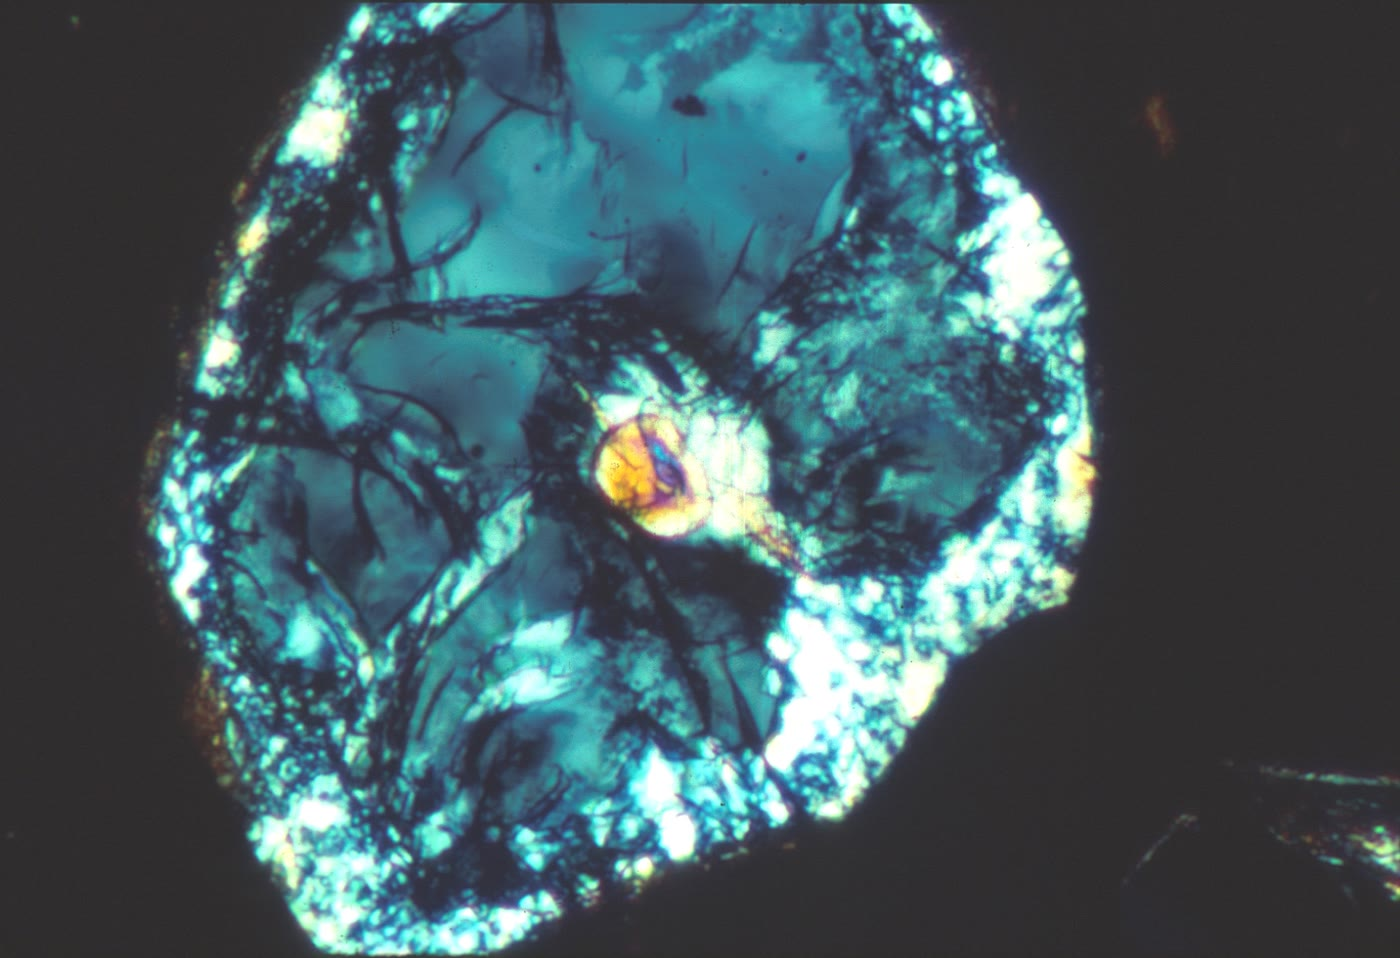
\includegraphics[width=0.62\linewidth]{images/book4/b2-11-coesite.jpg}
\par\smallskip{\small Koesit dalam eklogit, berukuran sekitar \qty{1}{mm}, dalam sayatan tipis
di antara polarisator bersilang: butir besar di tengah adalah koesit, tepi berupa butir-butir kecil yang terang adalah
kuarsa yang tumbuh darinya ketika tekanan turun; butir kecil berwarna di tengah adalah
inklusi piroksen. Foto: J.\,R. Smyth, CC BY-SA 1.0.}
\end{omfigure}

Enam tahun kemudian, intan berukuran rata-rata \qty{12}{\micro m} ditemukan dalam gneis, sekis, dan
batuan garnet--piroksen di masif Kokchetav di Kazakhstan utara, terselubung dalam garnet
dan zirkon, yang melindunginya dari perubahan menjadi grafit: intan itu tumbuh pada \qty{40}{kbar}
atau lebih dan di atas 900 sampai \qty{1000}{\celsius}. Kerak benua, betapapun ringannya, dapat
terseret turun lebih dari seratus kilometer.
% ledger: ss90:diamond

Bagaimana kerak itu kembali diceritakan oleh jam-jamnya. Di batuan terdalam yang tersubduksi di Alpen,
titanit yang diberi umur pada tahap-tahap berurutan menunjukkan bahwa sebuah batuan kalk-silikat mencapai sekitar
\qty{3.5}{GPa} pada $35.1 \pm \qty{0.9}{Ma}$, berada pada $1 \pm \qty{0.15}{GPa}$ pada $32.9 \pm
\qty{0.9}{Ma}$, dan di sekitar 0.4 sampai \qty{0.5}{GPa} pada $31.8 \pm \qty{0.5}{Ma}$. \omterm{def:b2:pt-paths:exhumation}{Laju
ekshumasi} rata-ratanya, 3.4 lalu \qty{1.6}{cm.yr^{-1}}, setara dengan kecepatan lempeng: batuan itu
kembali kira-kira secepat ketika turun, jauh lebih cepat daripada yang dapat dicapai erosi dalam mengupas
batuan di atasnya. Para penulisnya mengajukan daya apung, yaitu kerak ringan yang naik menembus mantel yang lebih rapat, dan
sesar normal, yang menipiskan batuan di atasnya.
% ledger: rh01:exhumation

\section{Metamorfisme dasar samudra}\label{sec:b2:pt-paths:ocean-floor}

\begin{definition}[Metamorfisme dasar samudra; serpentinisasi]\label{def:b2:pt-paths:ocean-floor}
Yang disebut \emph{metamorfisme dasar samudra}\index{metamorfisme dasar samudra} adalah
\omterm{def:b2:metamorphic-facies:metamorphism}{metamorfisme} regional litosfer samudra di dekat pusat pemekaran, oleh fluida berair panas
yang bersirkulasi di bawah gradien geotermal yang curam; rekristalisasinya umumnya tidak tuntas
dan suhunya biasanya naik dengan kedalaman. Yang disebut \emph{serpentinisasi}\index{serpentinisasi}
adalah hidrasi batuan kaya olivin menjadi serpentin.
\end{definition}
% ledger: scmr:types

Air laut yang tersedot ke dalam kerak muda di dekat sumbu punggungan memanas, bereaksi dengan batuan, dan
naik kembali. Basal yang dilaluinya terekristalisasi, secara tidak tuntas, menjadi mineral
hidrus, pada rentang suhu yang lebar. Di tempat air mencapai \omterm{def:b2:mantle-melting:peridotites}{peridotit}, seperti di
punggungan lambat tempat batuan mantel naik sampai ke dasar laut dan memasok mata air seperti
mata air di lapangan Lost City (volume Tahun 1), olivin mengikat air:
\[
\ce{2 Mg2SiO4 + 3 H2O -> Mg3Si2O5(OH)4 + Mg(OH)2},
\]
forsterit menghasilkan serpentin dan brusit. Volume molarnya, 43.65 untuk forsterit, 107.50
untuk serpentin, dan \qty{24.63}{cm^3.mol^{-1}} untuk brusit, menunjukkan akibatnya bagi batuan:
\qty{87.30}{cm^3} olivin menjadi \qty{132.13}{cm^3} padatan, \qty{51}{\percent}
lebih banyak, dan massa jenisnya turun dari 3.22 menjadi \qty{2.54}{g.cm^{-3}}. Batuan itu mengembang dan
menjadi lebih ringan, dan air yang diikatnya ikut turun bersamanya ketika lempeng itu tersubduksi.
% ledger: scmr:types, rh95:serpentine, kelley:lost-city, dick:ultraslow

\begin{inthelab}[Membaca sebutir garnet]
Untuk membaca \omterm{def:b2:pt-paths:paths}{lintasan P--T}, seorang petrolog pertama-tama membuat sayatan tipis melalui pusat
sebutir garnet, karena sayatan yang tidak melalui pusat akan melewatkan intinya. Di bawah mikroskop, inklusinya
dipetakan: butir-butir kecil kuarsa, biotit, plagioklas, atau kianit yang terperangkap ketika garnet
tumbuh, kadang-kadang berjajar dalam jejak yang mengawetkan foliasi batuan yang lebih tua. Mikroprobe
elektron kemudian mengukur komposisi di sepanjang garis dari inti ke tepi, dan peta
magnesium, besi, kalsium, dan mangan memperlihatkan zona-zona pertumbuhannya. Setiap zona dipasangkan dengan
mineral yang tumbuh bersamanya: inklusi untuk inti, matriks yang bersentuhan untuk
tepi. Termometer dan barometer diterapkan pada setiap pasangan, dan zona-zona itu diberi umur bila suatu
mineral memungkinkannya. \Cref{ch:b2:field-lab-methods-2} menguraikan instrumen-instrumennya.
\end{inthelab}

\begin{omfigure}
\centering
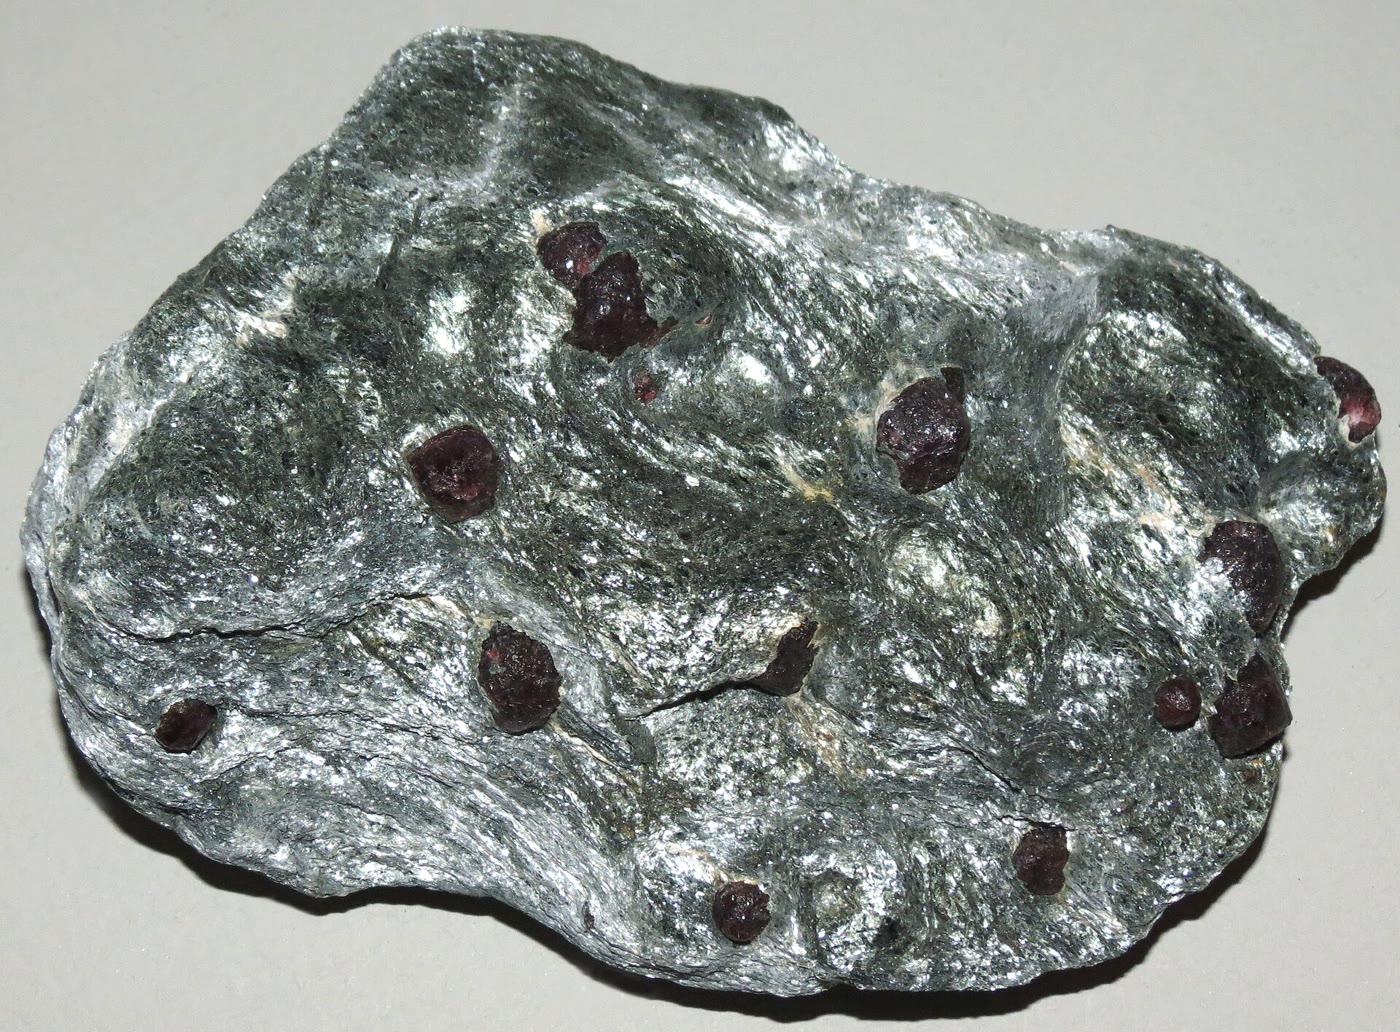
\includegraphics[width=0.62\linewidth]{images/book4/b2-11-garnet-schist.jpg}
\par\smallskip{\small Sekis garnet: kristal garnet merah tua yang tumbuh dalam matriks
mika yang berfoliasi. Setiap garnet dapat menyimpan, dari inti ke tepi,
rekaman lintasan batuannya. Foto: James St.~John, CC BY 2.0.}
\end{omfigure}

\section{Latihan}

\begin{exercise}[$\star$]\label{exo:b2:pt-paths:1}
Enam sampel dari satu formasi batu lumpur, yang dikumpulkan di sepanjang sebuah jalan, mengandung: (A) klorit,
muskovit, kuarsa; (B) biotit, klorit, muskovit, kuarsa; (C) garnet, biotit,
muskovit, kuarsa; (D) staurolit, garnet, biotit, muskovit, kuarsa; (E) kianit,
staurolit, biotit, muskovit, kuarsa; (F) silimanit, biotit, muskovit, kuarsa.
(a) Di \omterm{def:b2:pt-paths:barrovian}{zona Barrow} mana setiap sampel terletak? (b) Berapa isograd yang dilintasi jalan itu, dan
isograd yang mana? (c) Mengapa mengetahui isograd saja tidak cukup untuk menggambar \omterm{def:b2:pt-paths:barrovian}{gradien
metamorfik lapangan}?
\end{exercise}
% ledger: iugs:barrow

\begin{exercise}[$\star$]\label{exo:b2:pt-paths:2}
Sebutir garnet memiliki $X_{\text{Mg}} = 0.10$ dan $X_{\text{Fe}} = 0.80$, biotit di sampingnya
$X_{\text{Mg}} = 0.45$ dan $X_{\text{Fe}} = 0.50$. (a) Hitunglah $K_D$ dan $\ln K_D$.
(b) Dengan kalibrasi bab ini, hitunglah suhunya pada \qty{5}{kbar} dan pada
\qty{7}{kbar}. (c) Apakah hasil ini pengukur suhu atau pengukur tekanan?
\end{exercise}
% ledger: h97:ideal, h97:fs-reaction

\begin{exercise}[$\star$]\label{exo:b2:pt-paths:3}
Sebuah \omterm{def:b2:metamorphic-facies:protoliths}{metapelit} memberikan \qty{580}{\celsius} dan \qty{6.0}{kbar}. (a) Di bawah batuan bermassa jenis
rata-rata \qty{2800}{kg.m^{-3}} ($g = \qty{9.81}{m.s^{-2}}$), seberapa dalam letaknya? (b) Gradien
suhu berapa yang tersirat dari situ, mulai dari \qty{10}{\celsius} di permukaan? (c) Garis
eksperimental kianit $=$ silimanit melalui \qty{3.67}{kbar} pada
\qty{500}{\celsius} dan \qty{5.77}{kbar} pada \qty{600}{\celsius}: aluminosilikat mana
yang seharusnya dikandung batuan itu?
\end{exercise}
% ledger: hm93:table11

\begin{exercise}[$\star$]\label{exo:b2:pt-paths:4}
Untuk \omterm{def:b2:pt-paths:ocean-floor}{serpentinisasi} forsterit yang dituliskan dalam bab ini: (a) periksalah bahwa
persamaannya setara dalam massa, dengan massa molar 140.693 (forsterit), 18.015 (air),
277.112 (serpentin), dan \qty{58.320}{g.mol^{-1}} (brusit); (b) hitunglah perubahan
volume padatannya; (c) hitunglah massa jenis olivin dan massa jenis produknya.
(d) Apa akibat perubahan itu bagi \omterm{def:b2:mantle-melting:peridotites}{peridotit} terserpentinisasi di bawah dasar laut?
\end{exercise}
% ledger: rh95:serpentine

\begin{exercise}[$\star\star$]\label{exo:b2:pt-paths:5}
Kalibrasikan termometer itu dari empat percobaan pada \qty{2.07}{kbar}: $\ln K_D =
-1.157$ dan $-1.255$ pada \qty{799}{\celsius}, $-1.738$ dan $-1.826$ pada \qty{550}{\celsius}.
(a) Rata-ratakan setiap pasangan dan carilah garis $\ln K_D = a/T + b$ yang melalui kedua rata-rata itu.
(b) Turunkan $\Delta_r H$ dan $\Delta_r S$, dengan $\Delta_r V = \qty{0.311}{J.bar^{-1}}$.
(c) Bandingkan suhu yang diberikan kalibrasimu dan kalibrasi bab ini pada
\qty{5}{kbar} untuk $K_D = 0.18$, $0.10$, dan $0.30$. Apa kesimpulanmu tentang
ekstrapolasi suatu kalibrasi?
\end{exercise}
% ledger: h97:fs-data, h97:ideal

\begin{exercise}[$\star\star$]\label{exo:b2:pt-paths:6}
(a) Dari volume molar pada \qty{298}{K} (almandin 115.32, pirop 113.12, anit
154.30, flogopit 149.65, grosular 125.28, anortit 100.79, kianit 44.15, kuarsa
\qty{22.69}{cm^3.mol^{-1}}), hitunglah $\Delta_r V$ \omterm{def:b2:pt-paths:thermobarometry}{reaksi pertukaran} dan reaksi
GASP, lalu bandingkan dengan nilai yang dipakai kalibrasinya, \num{0.311} dan
\qty{-6.21}{J.bar^{-1}}. (b) Untuk $K_D = 0.18$, berapa kelvin galat sebesar
\qty{1}{kbar} menggeser suhunya? (c) Di sepanjang garis GASP sebuah batuan dengan
$X_{\text{Ca}}/X_{\text{an}} = 0.20$, berapa bar galat sebesar \qty{17}{K} menggeser
tekanannya?
\end{exercise}
% ledger: rh95:gb-gasp, rh95:al2sio5, h97:fs-reaction, kn88:gasp

\begin{exercise}[$\star\star$]\label{exo:b2:pt-paths:7}
Pada \qty{600}{\celsius}, sebutir garnet memiliki $X_{\text{Ca}} = 0.08$ dan plagioklas di sampingnya
$X_{\text{an}} = 0.30$. (a) Hitunglah tekanan GASP-nya. (b) Ulangi dengan $X_{\text{an}} =
0.35$. (c) Seberapa dalam letak batuan itu, untuk massa jenis rata-rata \qty{2800}{kg.m^{-3}}?
\end{exercise}
% ledger: kn88:gasp

\begin{exercise}[$\star\star$]\label{exo:b2:pt-paths:8}
Gunakan umur titanit batuan terdalam yang tersubduksi di Alpen: sekitar \qty{3.5}{GPa} pada
$35.1 \pm \qty{0.9}{Ma}$, \qty{1.0}{GPa} pada $32.9 \pm \qty{0.9}{Ma}$, \qty{0.45}{GPa} pada
$31.8 \pm \qty{0.5}{Ma}$. (a) Dengan massa jenis rata-rata \qty{3000}{kg.m^{-3}}, ubahlah
tekanan itu menjadi kedalaman. (b) Hitunglah kedua \omterm{def:b2:pt-paths:exhumation}{laju ekshumasi} rata-ratanya dan bandingkan dengan
nilai terbitan 3.4 dan \qty{1.6}{cm.yr^{-1}}. (c) Berapa ketidakpastian selang waktu
pertama, dan rentang laju mana yang dimungkinkannya? (d) Bandingkan dengan laju erosi
model penebalan, \qty{0.5}{mm.yr^{-1}}.
\end{exercise}
% ledger: rh01:exhumation

\begin{exercise}[$\star\star$]\label{exo:b2:pt-paths:9}
Untuk $K_D = 0.18$ pada \qty{5}{kbar}, (a) hitunglah $\partial T/\partial\ln K_D$ dan
$\partial T/\partial P$ dari proposisi itu; (b) dengan $\sigma_{\ln K_D} = 0.05$ (galat
\qty{5}{\percent} pada $K_D$) dan $\sigma_P = \qty{1}{kbar}$, hitunglah $\sigma_T$.
(c) Galat mana yang dominan? Bandingkan dengan ketidakpastian \qty{25}{\celsius} yang diklaim
untuk kalibrasi terbaik.
\end{exercise}
% ledger: h97:ideal

\begin{exercise}[$\star\star\star$]\label{exo:b2:pt-paths:10}
Tepi sebutir garnet memiliki $X_{\text{Mg}} = 0.10$, $X_{\text{Fe}} = 0.75$, $X_{\text{Ca}} = 0.07$;
biotit matriks $X_{\text{Mg}} = 0.42$, $X_{\text{Fe}} = 0.52$; plagioklas
$X_{\text{an}} = 0.25$. (a) Terapkan metode bab ini, mulai dari \qty{6}{kbar},
sampai suhunya berubah kurang dari \qty{1}{K}. (b) Aluminosilikat mana yang seharusnya dikandung
batuan itu (gunakan garis eksperimental \cref{exo:b2:pt-paths:3})? (c) Mengapa barometernya harus memakai
aluminosilikat yang benar-benar ada?
\end{exercise}
% ledger: h97:ideal, kn88:gasp, hm93:table11

\begin{exercise}[$\star\star\star$]\label{exo:b2:pt-paths:11}
Dengan $\kappa = \qty{1e-6}{m^2.s^{-1}}$: (a) hitunglah waktu relaksasi
proposisi itu untuk $L = \qty{35}{km}$ dan untuk $L = \qty{70}{km}$. (b) Model itu mengikis
\qty{35}{km} dalam 70 juta tahun; bandingkan waktu itu dengan kedua waktu pada (a). (c) Jelaskan,
dari waktu-waktu ini, mengapa batuan dalam model mencapai puncak termalnya setelah puncak
tekanannya. (d) Jika erosi sepuluh kali lebih cepat, apa yang akan berubah pada lintasannya?
\end{exercise}
% ledger: delaney:conductivity, et84:ptt

\begin{exercise}[$\star\star\star$]\label{exo:b2:pt-paths:12}
Ambillah kerak setebal \qty{35}{km} bermassa jenis \qty{2800}{kg.m^{-3}} di atas mantel bermassa jenis
\qty{3300}{kg.m^{-3}}. (a) Pada kedalaman berapa tekanan mencapai \qty{28}{kbar}, nilai
minimum bagi koesit Dora Maira? (b) Dan \qty{40}{kbar}, bagi intan Kokchetav?
(c) Gradien rata-rata berapa yang tersirat dari \qty{700}{\celsius} pada kedalaman (a), dan termasuk seri
mana? (d) Dengan \qty{3.4}{cm.yr^{-1}}, berapa lama pendakian dari kedalaman
(a) sampai \qty{35}{km}?
\end{exercise}
% ledger: chopin84:coesite, ss90:diamond, rh01:exhumation

\section{Soal: Perjalanan sebutir garnet}

\begin{problem}[{Soal akhir pekan --- termobarometri, lintasan, dan laju ekshumasi sebuah
sekis}]
\label{pb:b2:pt-paths:1}
Sebuah sekis kianit--garnet--biotit mengandung garnet yang memiliki inti dan tepi. Intinya menyelubungi
biotit, plagioklas, dan kianit; tepinya bersentuhan dengan biotit dan plagioklas
matriks. Di sekeliling garnet, sebagian kianit digantikan oleh silimanit, dan di pinggir
garnet tumbuh sedikit klorit. Hasil analisisnya adalah:
\begin{center}
\small
\begin{tabular}{@{}lccc@{}}
\hline
 & $X_{\text{Mg}}$ & $X_{\text{Fe}}$ & $X_{\text{Ca}}$ atau $X_{\text{an}}$\\
\hline
inti garnet & 0.080 & 0.760 & 0.050\\
biotit inklusi dalam inti & 0.40 & 0.58 & ---\\
plagioklas inklusi dalam inti & --- & --- & 0.25\\
tepi garnet & 0.120 & 0.720 & 0.060\\
biotit matriks & 0.46 & 0.53 & ---\\
plagioklas matriks & --- & --- & 0.28\\
\hline
\end{tabular}
\end{center}
Gunakan termometer garnet--biotit dan barometer GASP bab ini (pencampuran ideal),
$R = \qty{8.314}{J.mol^{-1}.K^{-1}}$, $g = \qty{9.81}{m.s^{-2}}$, massa jenis rata-rata
\qty{2800}{kg.m^{-3}} di atas batuan, dan bulatkan setiap rasio sampai empat desimal.

\noindent\textbf{Bagian I --- Suhu.}
\begin{enumerate}
\item Hitunglah $X_{\text{Mg}}/X_{\text{Fe}}$ dalam inti garnet dan dalam biotit
inklusi, lalu $K_D$ dan $\ln K_D$ untuk inti.
\item Lakukan hal yang sama untuk tepi dan biotit matriks.
\item Hitunglah suhu inti pada \qty{6}{kbar}.
\item Hitunglah suhu tepi pada \qty{6}{kbar}.
\item Berapa kelvin galat sebesar \qty{1}{kbar} akan mengubah suhu-suhu ini?
\item Mengapa inti dipasangkan dengan biotit inklusi, dan tepi dengan biotit
matriks?
\end{enumerate}

\noindent\textbf{Bagian II --- Tekanan.}
\begin{enumerate}[resume]
\item Hitunglah tekanan anggota ujung $P_0$ reaksi GASP pada kedua suhu
pertanyaan~3 dan~4.
\item Hitunglah tekanan GASP inti pada suhu pertanyaan~3.
\item Hitunglah tekanan GASP tepi pada suhu pertanyaan~4.
\item Hitung ulang suhu tepi pada tekanan pertanyaan~9, lalu tekanannya
pada suhu itu, dan sekali lagi suhunya. Berikan suhu dan tekanan
tepi.
\item Lakukan hal yang sama satu kali untuk inti. Mengapa hasilnya hampir tidak berubah?
\item Ubahlah tekanan inti dan tepi menjadi kedalaman.
\item Garis eksperimental kianit $=$ silimanit melalui 3.67, 5.77, dan
\qty{7.86}{kbar} pada 500, 600, dan \qty{700}{\celsius}. Aluminosilikat mana yang stabil
ketika inti tumbuh, dan ketika tepi tumbuh? Apakah kianit di inti konsisten?
\end{enumerate}

\noindent\textbf{Bagian III --- Lintasannya.}
\begin{enumerate}[resume]
\item Di antara inti dan tepi, seberapa besar suhu dan tekanan berubah?
Apakah garnet tumbuh pada \omterm{def:b2:pt-paths:paths}{lintasan progradasi} atau retrogradasi?
\item Silimanit menggantikan kianit di sekeliling garnet. Pada suhu tepi,
di bawah tekanan berapa batuan itu harus lewat agar hal itu terjadi? Apa yang dialami batuan itu
setelah tepinya tumbuh?
\item Klorit tumbuh di pinggir garnet. Bagian lintasan mana yang direkamnya?
\item Gambarlah lintasannya: inti, tepi, silimanit, klorit. Apakah searah atau berlawanan arah jarum jam?
Puncak mana yang datang lebih dulu?
\item Model penebalan bab ini membawa batuannya ke puncak termal
\qty{593}{\celsius} pada \qty{7.8}{kbar}. Apakah lintasan sekis ini sejenis?
\end{enumerate}

\noindent\textbf{Bagian IV --- Seberapa cepat.}
\begin{enumerate}[resume]
\item Tepi garnet memberikan umur samarium--neodimium $412.0 \pm \qty{1.5}{Ma}$, yang dianggap
sebagai umur puncak; sebutir muskovit matriks memberikan umur argon $398.0 \pm
\qty{1.0}{Ma}$, yaitu waktu ketika batuan itu mendingin melewati \qty{405}{\celsius}. Hitunglah
laju pendinginan rata-rata di antara keduanya.
\item Suhu penutupan \qty{405}{\celsius} mengandaikan pendinginan sebesar
\qty{10}{\celsius} per juta tahun. Apakah laju pada pertanyaan~19 menuntut nilai yang lebih tinggi atau
lebih rendah, dan mengapa?
\item Pada \qty{398}{Ma}, ambillah geoterm \qty{30}{\celsius\per\km} mulai dari
\qty{10}{\celsius} di permukaan. Pada kedalaman berapa muskovit itu menutup?
\item Seberapa jauh batuan itu naik antara puncak dan penutupan muskovit?
\item Berapa ketidakpastian selang waktunya?
\item Hitunglah \omterm{def:b2:pt-paths:exhumation}{laju ekshumasi} rata-rata dari puncak sampai penutupan muskovit, dalam
milimeter per tahun dan dibulatkan sampai sepersepuluh: angka kunci soal ini.
\end{enumerate}
\end{problem}
% ledger: h97:ideal, h97:fs-reaction, kn88:gasp, hm93:table11, h09:muscovite, scmr:ptt, et84:ptt
